\chapter{Descripción del problema}

En este capítulo se detallará el problema que se pretende resolver con este proyecto, además de establecer los objetivos que se requieren cumplir. Se realizará una crítica al estado del arte y para finalizar se enunciará una propuesta de producto.

\section{Problema a resolver}
Como se ha comentado en apartados anteriores, existen en el mercado multitud de experiencias de Realidad Aumentada al alcance de los usuarios, aunque en la gran mayoría de ellas los usuarios juegan un rol pasivo. Esto último no hace referencia a que no puedan interactuar con el contenido, (ya hemos visto que la interacción en tiempo real es uno de los rasgos definitorios de la \textit{RA}) sino que consumen contenidos y experiencias que han sido creadas por los desarrolladores de las distintas apps. Suelen ser sistemas cerrados donde el usuario no tendría opción de, por ejemplo, cargar un modelo 3D de su dispositivo para visualizarlo en su salón.

Por otro lado, las herramientas de modelado y animación de objetos 3D como \textit{Blender}\footnote{https://www.blender.org/} o \textit{https://www.autodesk.es/products/3ds-max/overview}\footnote{link 3ds max} son herramientas profesionales que requieren de una formación, conocimientos previos y curva de aprendizaje para poder manejarlos con soltura. Incluso si las aplicaciones pudieran efectivamente cargar modelos en las aplicaciones ya mencionadas, estarían limitados a elementos sueltos que pudieran encontrar en internet. Esto es algo que limita mucho tus opciones creativas. Volviendo al ejemplo de la escena del parque que se puso en el capítulo 1, si se pretende recrear hacer la escena de un parque, quizás se encuentre un modelo 3D para ello. Pero, ¿y si se quiere tenga concretamente dos toboganes y un columpio? Es muy poco probable que alguien haya modelado y publicado una escena con exactamente los mismos requisitos. Pero contando con que se puedan encontrar los elementos por separado (un modelo de un tobogán, de un balancín, de un columpio...) lo cual es más realista, y alguna forma de componerlos en una sola escena, se podría construir un parque con una composición cualquiera.

Teniendo todo esto en cuenta se detectan dos necesidades para el usuario. Por un lado, una suerte de editor sencillo, simplificado e intuitivo en el que un usuario sin conocimiento o experiencia previa pueda cargar o crear modelos 3D con los que pueda construir una escena con total libertad creativa. Por otro lado, una manera de que el usuario pueda reproducir cómodamente sus composiciones producidas en un contexto de Realidad Aumentada en un dispositivo con cámara como podría ser un \textit{smartphone}.

Este escenario presenta ciertos retos de diseño e implementación. El software profesional de modelado profesional es complejo por una razón: tienen muchísimas posibilidades. Si se quiere tener una herramienta sencilla inevitablemente el usuario perderá opciones. Por tanto, se debe encontrar un compromiso, un \textit{sweetspot} en el que se intenten cubrir casi todas las necesidades que podría tener una persona sin que el software se vuelva demasiado obtuso. También se debe de tener en cuenta un aspecto técnico importante: qué formato de archivos para modelos soportará el sistema. Existe una gran variedad hoy en día, cada uno con sus peculiaridades, y no siempre compatibles entre ellos, por lo que el software deberá adoptar uno o contar con herramientas de conversión para soportar un conjunto de ellos. También hay que tener en cuenta que el tipo de dispositivo en el que principalmente se tiene interés por reproducir escenas \textit{RA} son teléfonos móviles o tablets debido a sus cámaras integradas y su portabilidad, pero estos se controlan con gestos táctiles, los cuales no son tan precisos como un ratón de ordenador y podría ser una dificultad a la hora de implementar controles precisos para el editor. Por ello deberá buscarse una forma de adaptar este tipo de programa a un control táctil o bien implementar una conectividad ordenador-\textit{smartphone} para poder crear la escena en el primero y reproducirla en el segundo. En este TFG se propondrá y desarrollará una solución para estas necesidades.

\section{Objetivos}

Una vez definidos los retos y problemas a resolver en este contexto, se procede a enunciar los objetivos a los que se pretende llegar con este proyecto:

\begin{itemize}
    \item \textbf{OBJ-1}: Desarrollar un software que permita cargar y crear modelos 3D a los que aplicarles transformaciones como translaciones, rotaciones y escalado para construir una escena.
    \item \textbf{OBJ-2}: El software descrito descrito debe ser simple, sencillo e intuitivo para que lo pueda usar cualquier persona sin que tenga experiencia ni conocimientos previos en la materia.
    \item \textbf{OBJ-3}: El software debe permitir la máxima flexibilidad posible a la hora de producir las escenas teniendo en cuenta su alcance limitado y controles sencillos.
    \item \textbf{OBJ-4}: Desarrollar una aplicación informática que reciba como entrada uno o varios modelos 3D que compongan una escena y reproduzca con ellos una experiencia de realidad aumentada.
    \item \textbf{OBJ-5}: El sistema debe tener memoria, es decir, un usuario deberá de alguna forma poder conservar las escenas generadas con anterioridad para que el usuario las pueda volver a modificar en un futuro.
\end{itemize}

\section{Estado del arte}

Existe en el mercado cierta variedad de opciones desarrolladas que cumplen en mayor o menor medida los objetivos que se han planteado en este TFG. Esta sección se dedicará a analizarlas, compararlas y detectar cuales son las fortalezas y carencias de cada una, con la intención de sacar en claro qué se podría aportar con una nueva solución. Después de investigar y analizar las soluciones más relevantes, se encontraron \textbf{cinco plataformas} con un propósito y características similares al proyecto que se pretende desarrollar. De estas cinco se descartaron dos, \textit{Aryel}\footnote{\url{https://aryel.io/}} y \textit{Artificio}\footnote{\url{https://arficio.com}} ya que aunque superficialmente comparten algunos elementos como son al fin de al cabo la creación de escenas \textit{RA}, la primera está enfocada para que se le dé uso en agencias de marketing para diseñar publicidad interactiva, y la segunda es una herramienta para diseñar interiores de viviendas.

\subsection{Onirix Studio}
\textit{Onirix Studio}\cite{onirix} (figura \ref{onirix}) es una plataforma gratuita en la que un usuario al darse de alta puede crear multitud de escenas \textit{RA} a través de un editor. Las escenas producidas quedan registradas en la cuenta de usuario, y pueden ser accedidas a través de un menú que permite volver a editarlas o eliminarlas. En cuanto al editor tiene un gran abanico de opciones. El usuario puede añadir modelos a la escena, posicionarlos, rotarlos y escalarlos con total libertad a través tanto de controles gestuales de ratón como de un panel numérico. Cuenta con la posibilidad de modificar la iluminación que proyecta la escena sobre los modelos. Es posible añadir texto que se visualice junto a los modelos. Para añadir \textit{assets} como los modelos, el usuario cuenta con un catálogo personal, con algunos elementos que añade la aplicación por defecto, pero con la opción de que el usuario añada los suyos propios. Una vez los añade los puede usar en cualquier otro proyecto.

\begin{figure}[h]
    \centering
    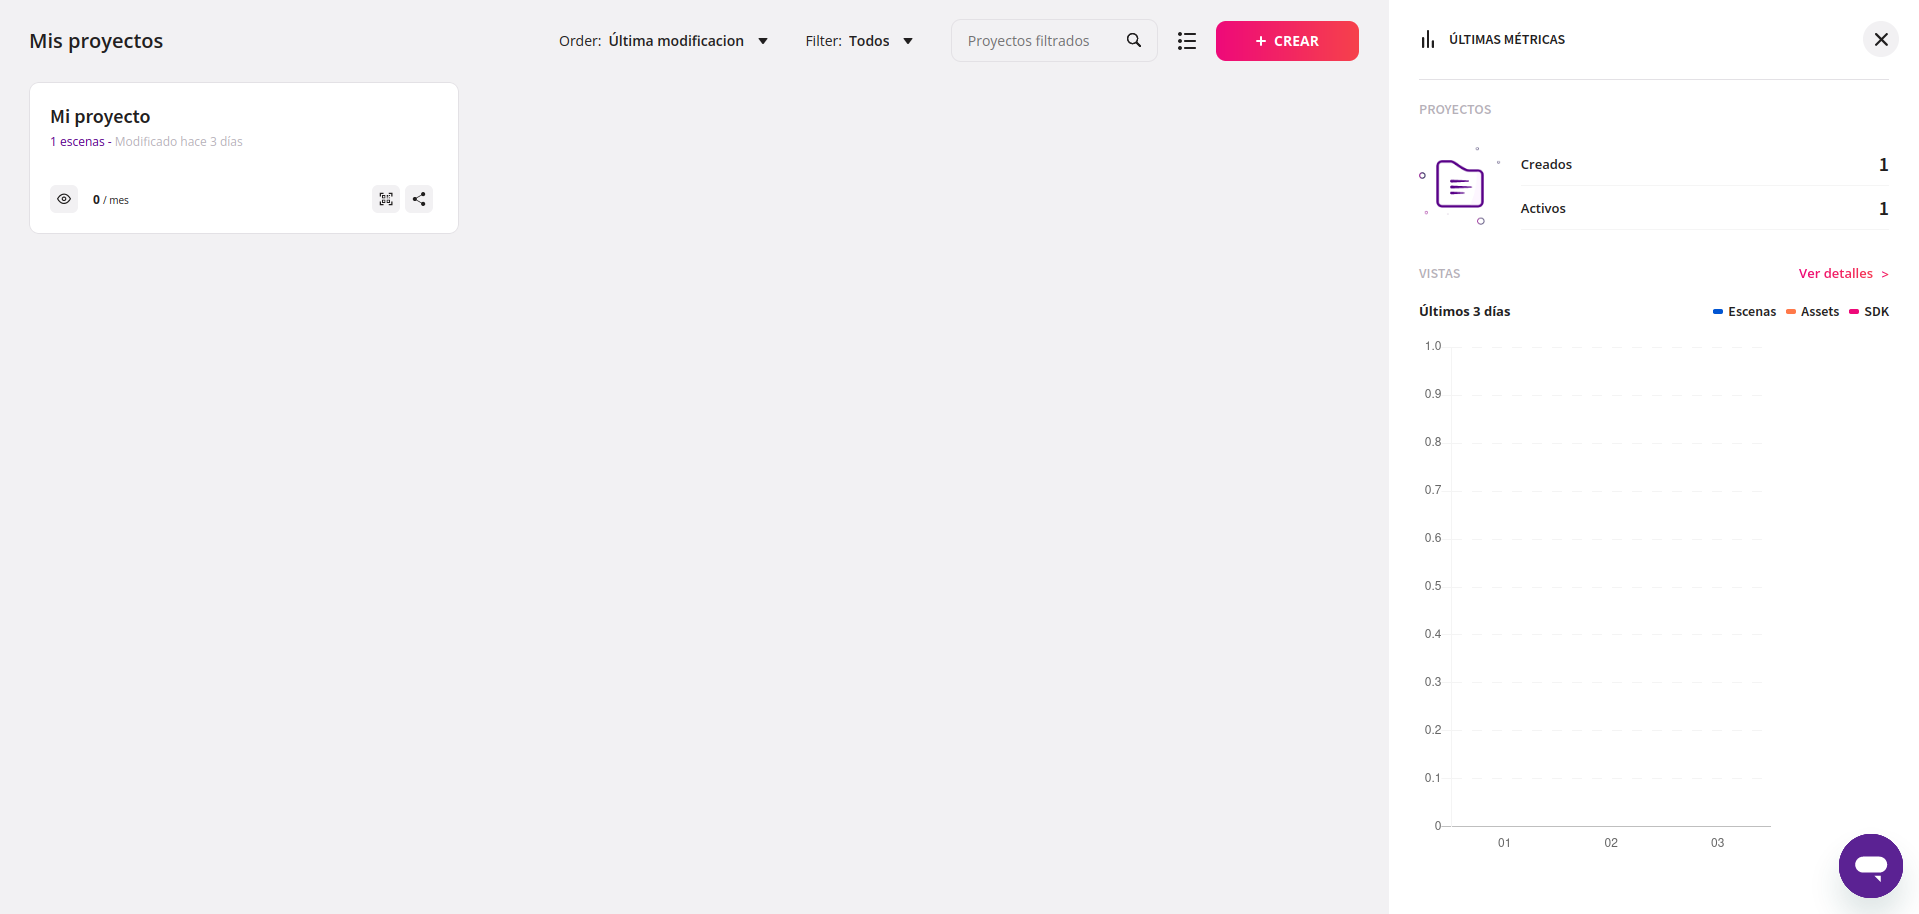
\includegraphics[scale=0.27]{onirix1}
    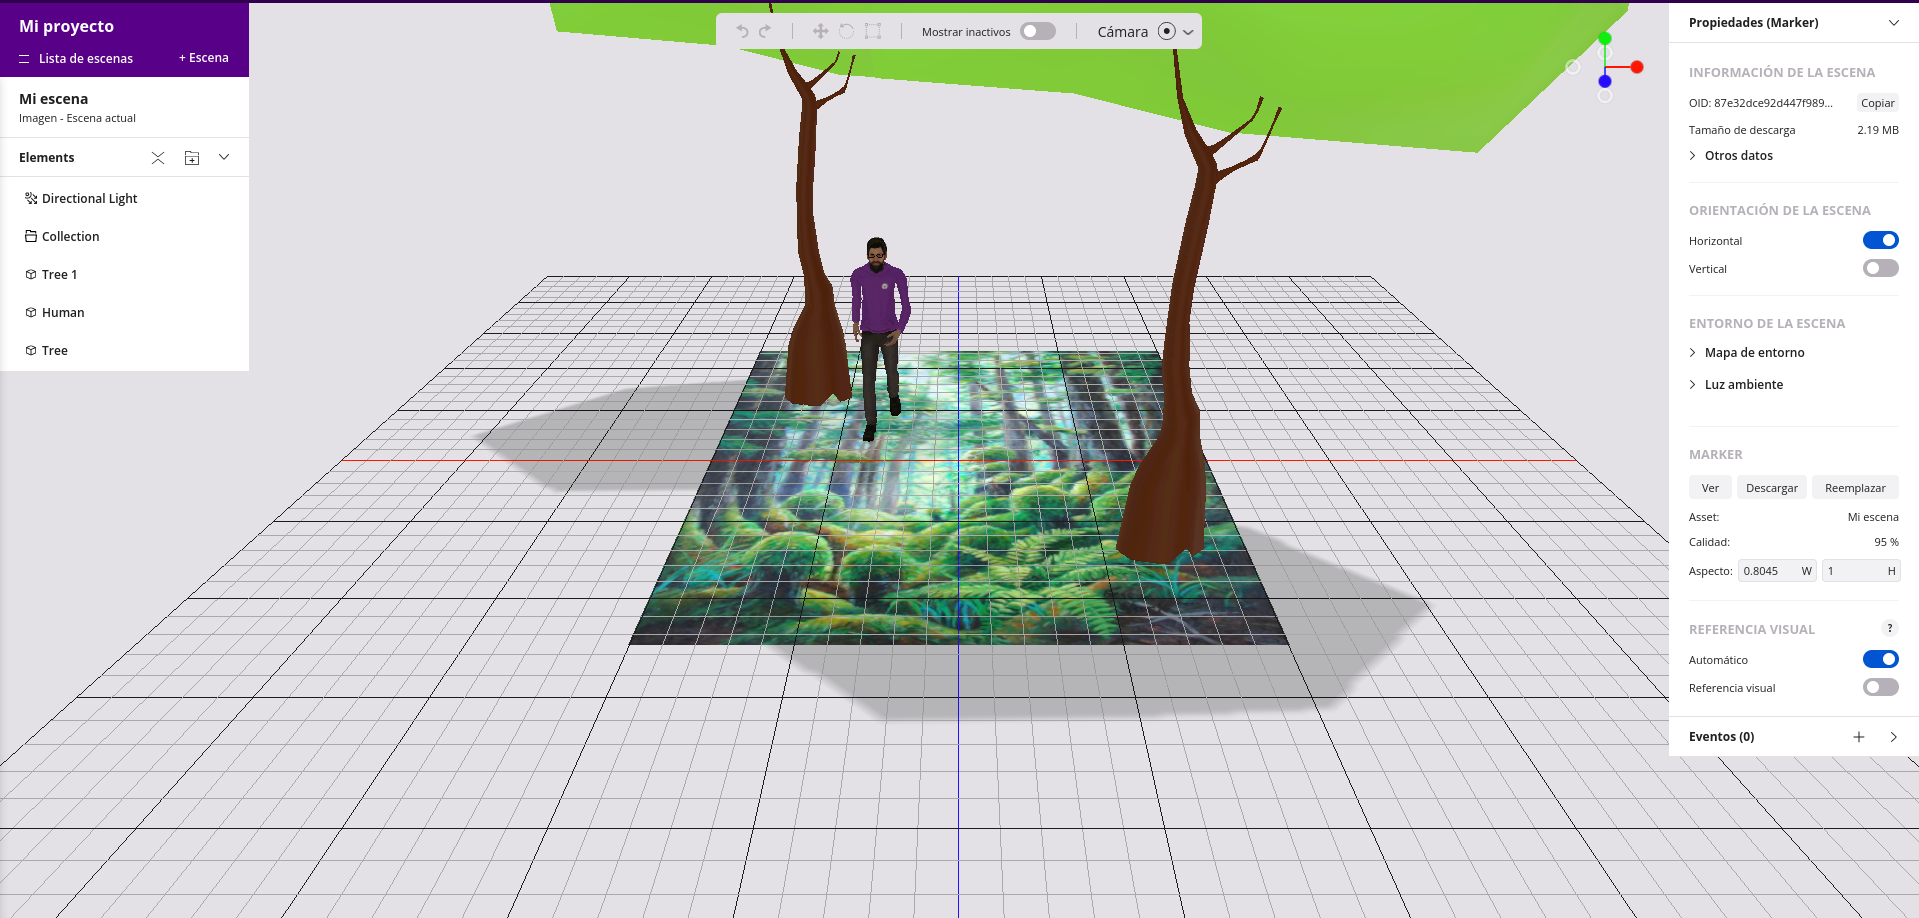
\includegraphics[scale=0.27]{onirix2}
    \caption[Aplicación Onirix Studio]{Web de creación de escenas RA Onirix Studio}
    \label{fig:onirix}
\end{figure}

Uno de los puntos más destacables que ofrece este entorno es un sistema al través del cual se pueden definir eventos dinámicos para la escena al cumplirse cierto activador. Por ejemplo, si tenemos un botón pulsable en la escena, se puede añadir una regla que ordena al pulsarse el botón la reproducción de la animación de uno de los modelos, o aparezcan modelos nuevos, desaparezcan otros, etc.

Para la reproducción tenemos se pueden o bien reproducir en la propia web, o generar un \textit{código QR} escaneable por un \textit{smartphone}. Este \textit{QR} abre en el navegador un enlace a través del cual se reproduce la escena. Por un lado, esta es una solución cómoda y ágil, pero tiene puntos negativos. Para empezar el rendimiento de la cámara y renderización de elementos 3D de un dispositivo móvil se va a ver reducida si es a través de una aplicación web en lugar de una aplicación nativa del teléfono. También hay que tener en cuenta que existe un enorme catálogo de navegadores gratuitos, y aunque la mayoría de los usuarios utilizan los más populares como \textit{Google Chrome}, \textit{Mozilla Firefox}, \textit{Opera} o \textit{Safari}, no se puede asegurar la compatibilidad total con cualquier navegador, o que el rendimiento sea óptimo en todos. Otro punto negativo a destacar de \textit{Onirix Studio}\cite{onirix} es que solo es posible crear escenas de posicionamiento sobre superficie y de imágenes aumentadas.

\subsection{Blippbuilder}

\textit{Blippbuilder}\cite{blippbuilder} (figura \ref{bipp}) es una web muy similar a la anteriormente comentada, y también se puede emplear sin coste alguno. A través de una cuenta el usuario puede almacenar una colección de escenas RA editables a través de un menú similar. El editor contaba con una estructura parecida, permitiendo también aplicar transformaciones con gestos de ratón. Al igual que la anterior, tiene la opción tanto de cargar recursos desde el ordenador del usuario como de acceder a una librería incluida con la web, opción de añadir texto, manipular la iluminación de la escena. También cuenta con un pre visualizador dentro del editor y con opción para probar la escena desde el navegador de un dispositivo móvil escaneando un código \textit{QR} (es decir, tampoco es nativa).

\begin{figure}[h]
    \centering
    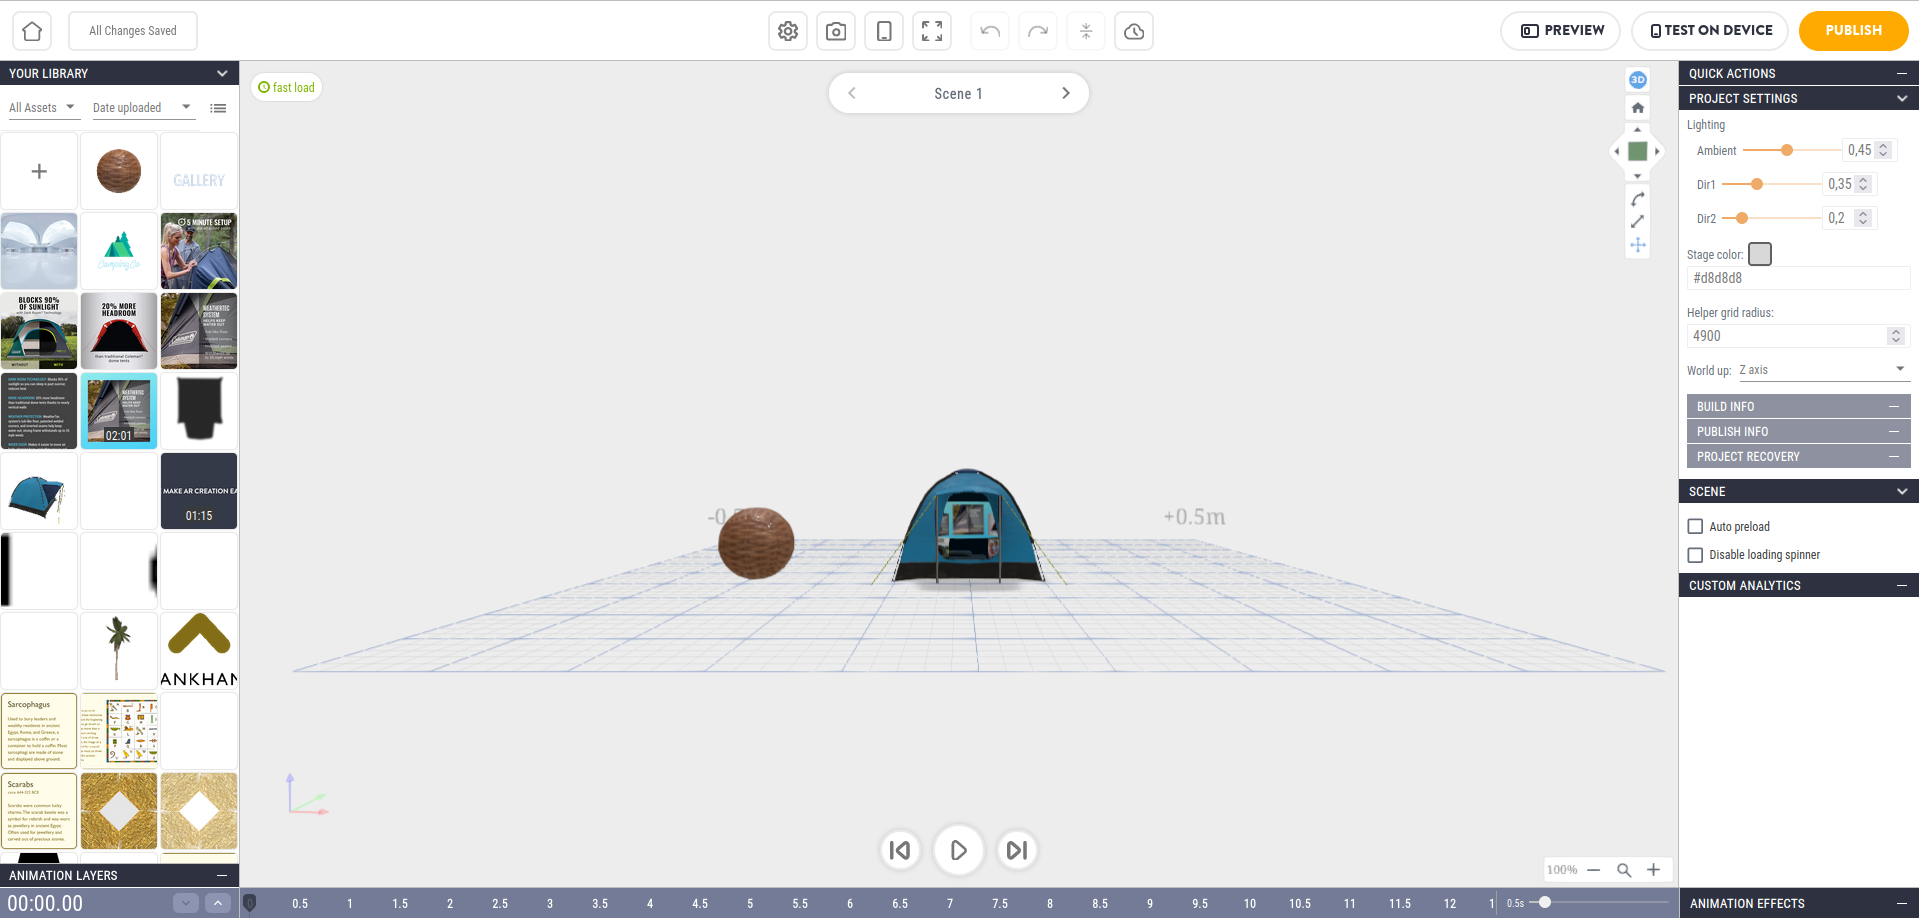
\includegraphics[scale=0.27]{bipp1}
    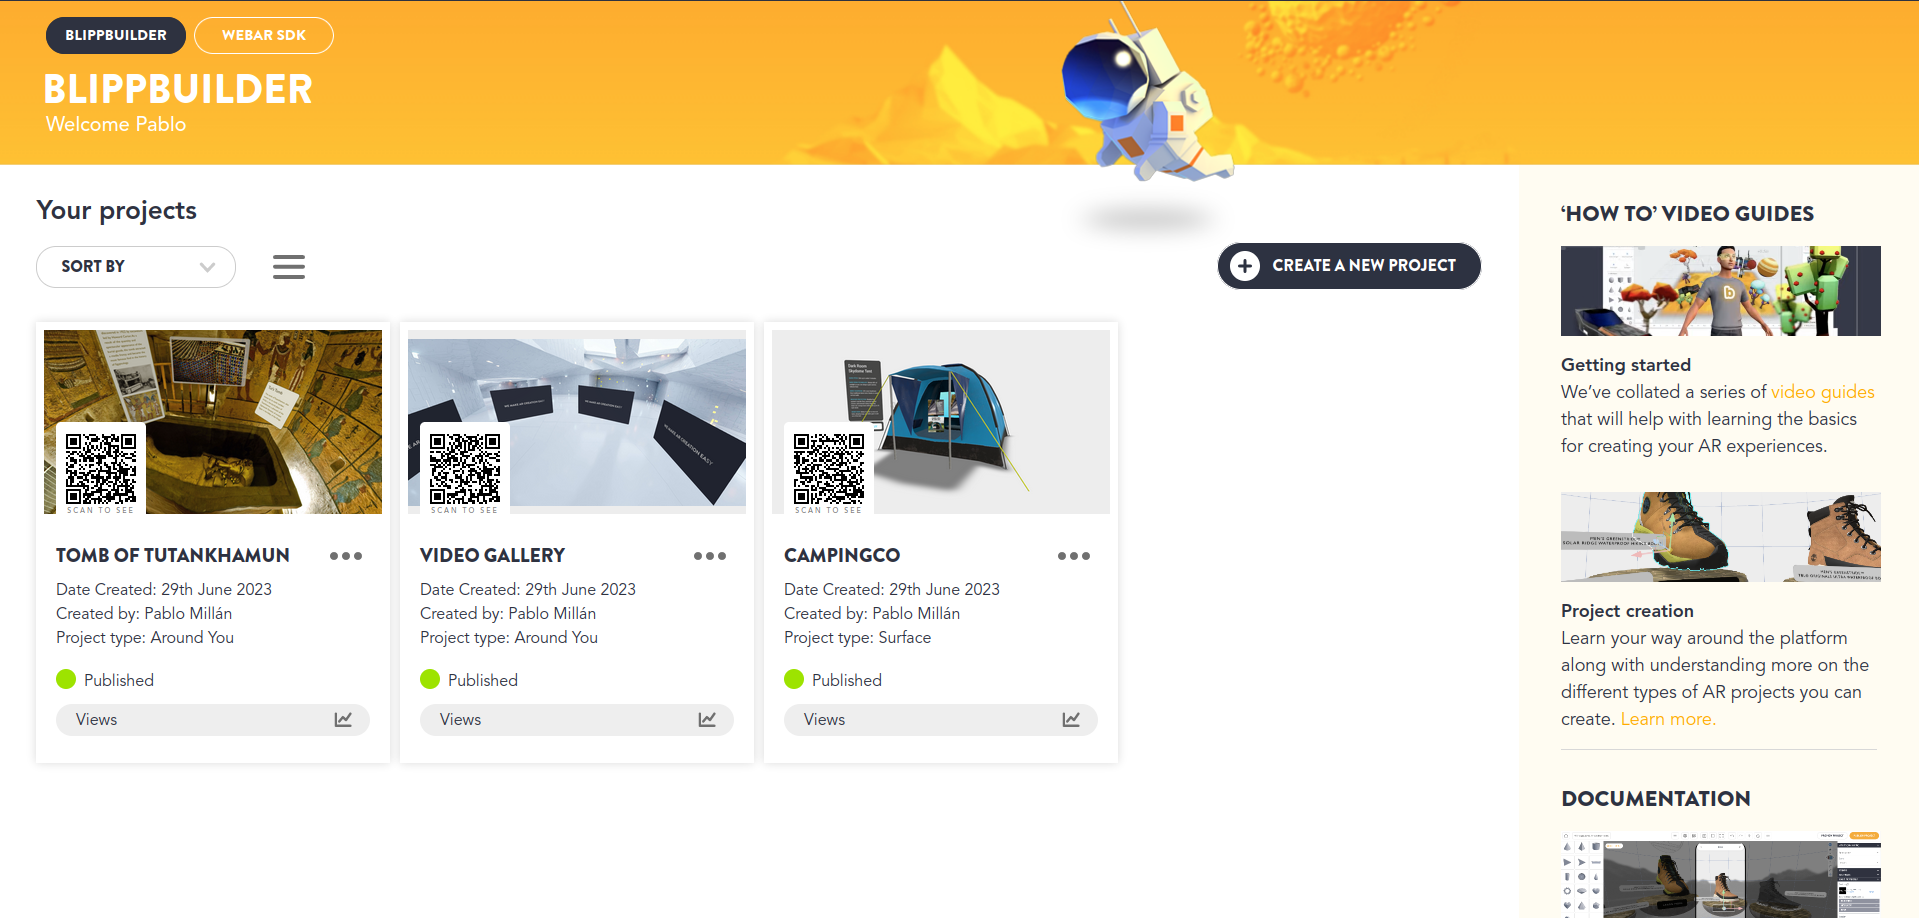
\includegraphics[scale=0.27]{bipp2}
    \caption[Aplicación BlippBuilder]{Web de creación de escenas RA BlippBuilder}
    \label{fig:bipp}
\end{figure}

Como aspecto diferenciador, es posible añadir a la escena geometrías básicas tales como esferas, cubos o cilindros para añadirlos. Además, cuenta con un menú a través del cual se pueden \textbf{crear animaciones} para la escena. A través de \textit{keyframes}. Un \textit{keyframe} o \textit{fotograma clave} es una unidad de información que almacena atributos tales como la posición, rotación o escala de un objeto para un instante determinado. Definiendo dos \textit{keyframes} para el mismo objeto en 2 instantes distintos, un software puede interpolar sus posiciones intermedias generando así una animación. Esta animación puede ser reproducida junto a la escena.

En \textit{Blippbuilder} solo es posible la creación de escenas de Realidad Aumentada por superficie.

\subsection{Pictarize}
\textit{Pictarize}\cite{pictarize} (figura \ref{pictarize}) de nuevo tiene un funcionamiento muy parecido a lo visto hasta ahora y sin requerir de pagos. Una galería de escenas producidas asociadas a una cuenta de usuario, y un editor para hacer las mismas. Tiene opción para cargar modelos desde el ordenador del cliente y de nuevo controles gestuales con el ratón para manipularlos. Aunque también puede añadir texto, no existe opción para alterar la iluminación. Sin embargo, es posible embeber videos de youtube en forma de textura plana, para reproducirlos al pulsarlos cuando se reproduce la escena. Es posible también asociar una pista de audio a la escena para que se reproduzca junto a las animaciones de los modelos 3D.

\begin{figure}[h]
    \centering
    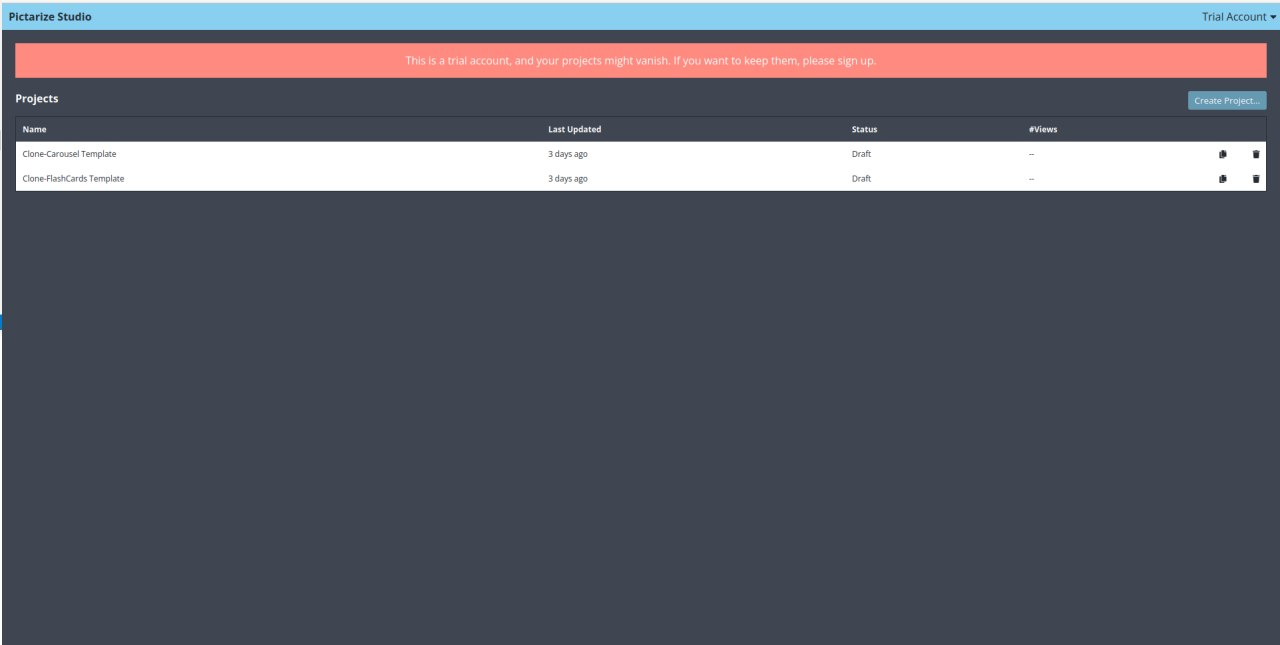
\includegraphics[scale=0.4]{pic1}
    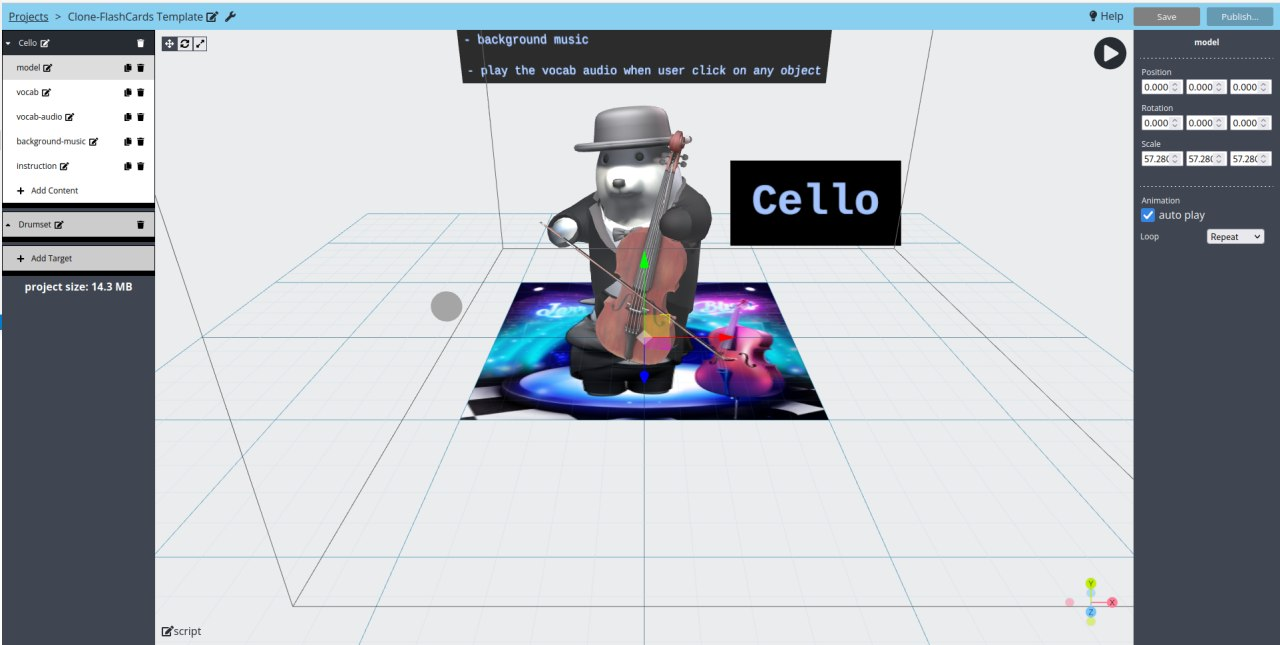
\includegraphics[scale=0.4]{pic2}
    \caption[Aplicación Pictarize Studio]{Web de creación de escenas RA Pictarize Studio}
    \label{fig:pictarize}
\end{figure}

Para la reproducción de escenas se cuenta tanto con un pre visualizador dentro del editor como una opción para verlas desde un \textit{smartphone} a través de un código \textit{QR} y un navegador web, como se ha visto en los dos ejemplos anteriores. Sólo hay opción para escenas de imágenes aumentadas, con la opción de definir distintos activadores para distintos elementos.

\section{Crítica}

Como se ha podido dilucidar a través de estos ejemplos ya hay varias soluciones disponibles y bastante completas aun siendo gratuitas. Sus editores son potentes en cuanto a que permiten un alto grado de expresión por parte del usuario, permitiendo un gran abanico de posibilidades de forma que el usuario podrá muy probablemente representar la escena que tenía en mente siemrpe que cuente con los modelos adecuados.

Las propuestas existentes analizadas comparten multitud de elementos en común. Todas ofrecen un menú para gestionar una lista de escenas creadas por un usuario, el cual se identifica con una cuenta para la propia web. Esta cuenta usa como identificador un nombre de usuario y correo electrónico. En todas es posible cargar objetos 3D desde el ordenador del cliente.

También permiten aplicar transformaciones de translación, rotación y escalado a los modelos de la escena con gestos del ratón a través de \textit{gizmos} ((figura \ref{gizmo})). Estos son unas estructuras visuales interactuables que ayudan a aplicar transformaciones a objetos 3D. Dependiendo de la operación que se quiera realizar, hay distintos tipos de gizmo. Cogiendo el ejemplo del \textit{3D Move Gizmo} de la siguiente figura, si se hiciera click en una de las flechas coloreadas, se permitiría mover el objeto con un desplazamiento del ratón en el eje que señala la misma. Además de controles gestuales permiten introducir manualmente números para representar las transformaciones del objeto a través de un menú. Por ejemplo se puede especificar que un modelo está \textit{'6.2' unidades desplazado en el eje X} o con \textit{una rotación de 90º en el eje Y}.

\begin{figure}[h]
    \centering
    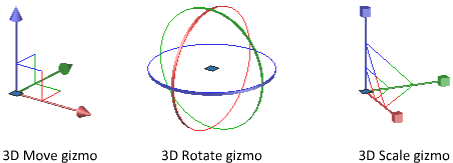
\includegraphics[scale=1.0]{gizmo}
    \caption[Gizmo en Autodesk AutoCAD]{Ejemplo de Gizmo en la documentación de Autodesk}
    \label{fig:gizmo}
\end{figure}

Hay otras funciones que si bien no son imprescindibles para el objetivo de crear una escena, dan posibilidades extra de personalización como la adición de texto, manipulación de luces, reproducción de audios, definición de eventos o creación de animaciones con \textit{keyframes}. Hay que tener una cosa en cuenta con este tipo de funcionalidades, y es que si bien aportan valor y posibilidades a la aplicación, también aumentan la complejidad de la aplicación y la curva de aprendizaje que tienen los usuarios. No es descabellado pensar que alguien que no tiene nociones básicas sobre cómo funciona la animación tenga dificultades para manipular una timeline de \textit{fotogramas clave} para crear una pequeña animación. Por tanto, se puede deducir que un porcentaje de los usuarios se sentirán confundidos por funciones como esta o la de definir eventos, o directamente no llegarán a intentar usarla.

También hay presentes algunas carencias en estas webs. Se puede ver que una de ellas permite crear tanto escenas por superficie como de imágenes aumentadas, mientras que en las otras dos opciones solo es posible hacer o imágenes aumentadas o superficie. Y lo que es más, ninguna tiene soporte para generar escenas geoespaciales basadas en la localización.

Otra ausencia a destacar es la imposibilidad en ninguna propuesta de descargar guardar de forma local en el ordenador las escenas que se han creado en un formato de objeto 3D, para que el usuario pueda utilizar ese archivo en cualquier otro software que admita el tratamiento de modelos. Esto se traduce en una imposibilidad de que las escenas salgan del ecosistema de sus respectivas webs.

Por último señalar que en todas las webs analizadas la única opción para reproducir las escenas en un entorno real de Realidad Aumentada en un dispositivo móvil es a través de un navegador web al que se accede escaneando un código QR. Como se ha explicado anteriormente, se trata de una opción cómoda en tanto que es multiplataforma, no hace falta iniciar sesión de nuevo en el segundo dispositivo y en pocos segundos se puede escanear el código y tener cargando la escena, pero el rendimiento y fluidez de la cámara que se obtiene es considerablemente menor que si estuviera corriendo en una aplicación nativa, por lo que no estaría de más tener la opción de ejecutarlo de esta forma.

\section{Propuesta}

Con esta propuesta de proyecto se pretende desarrollar una alternativa completa que intentará cubrir las carencias que se encontraron analizando las webs disponibles en el mercado:

\begin{itemize}
    \item \textbf{Intuitivo}: El editor contará con las herramientas básicas e imprescindibles para poder elaborar una escena 3D con las necesidades del usuario. Esto permitirá mantener una interfaz limpia, legible e intuitiva que permita construir escenas de una forma rápida y que no requiera conocimientos o experiencias previas con software de manipulación de entornos 3D. Así los usuarios no se sentirán perdidos o que tiene más herramientas de las que realmente necesitan.
    \item \textbf{Múltiples tipos de escenas}: Será posible la creación de distintos tipos de escenas de Realidad Aumentada. En concreto permitirá escenas de posicionamiento por superficies, de imágenes aumentadas y geoespaciales en unas coordenadas concretas.
    \item \textbf{Descarga de escenas}: Además de poder almacenar las creaciones en la nube, será posible exportar la escena con formato de objeto 3D para que el usuario pueda emplearla en cualquier otro software que permita archivos de este tipo.
    \item \textbf{Reproducción nativa}: Será posible reproducir escenas en una aplicación nativa para dispositivos móviles, proporcionando un mayor rendimiento y asegurando compatibilidad.
\end{itemize}

Para eso se desarrollará un servicio completo que contará de tres partes fundamentales. Para empezar, una \textbf{aplicación web} que permita la creación y gestión de escenas de realidad aumentada. Por otro lado, se tiene una \textbf{aplicación móvil} desde la que reproducir de forma nativa las escenas. Para terminar, un \textbf{servidor web} en el que se almacenarán las escenas creadas, que podrán ser recuperadas tanto desde la aplicación web como la aplicación móvil.

En el capítulo 4 se dará una hablará más en detalle del software en una descripción del mismo desde el ángulo de las metodologías ágiles, y en el capítulo 5 se explicará tanto la implementación como las decisiones de diseño y tecnologías empleadas.